\section{CD-SAXS}
\subsection{Introduction}

\medskip

Miniaturizing transistors, the building blocks of integrated circuits, is getting
tougher for the semiconductor industry. Shrinking their size and spacing (pitch)
brings not only manufacturing hurdles but also a metrology problem. Precisely
measuring these features during production is crucial for high-quality chips.
Existing in-line metrology techniques, like optical critical-dimension (OCD)
scatterometry and critical-dimension scanning electron microscopy (CD-SEM), are
nearing their limits \cite{SEM_resolution,OCD_resolution}. OCD struggles with limitations inherent to light and the
ever-shrinking features. CD-SEM offers valuable insights because it provides an image of the sample but is restricted by
the sampling area and also its resolution. To overcome these obstacles, the industry is exploring X-ray-based metrology.
X-rays have much shorter wavelengths than the features being measured, allowing
for more precise analysis. Additionally, they are sensitive to variations in
composition, providing a richer data set.

\begin{figure}[h]
    \centering
    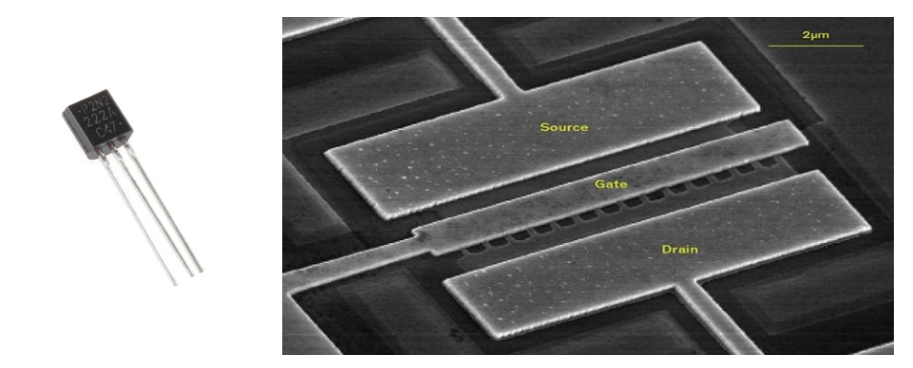
\includegraphics[width=0.6\textwidth]{images/transistor.png}
    \caption{A classic transistor with three terminals. (On the right, an electron microscope image of a single transistor on a microchip.)\cite{transistor}}
    \label{fig:transistor}
\end{figure}

\medskip


\begin{figure}
    \centering
    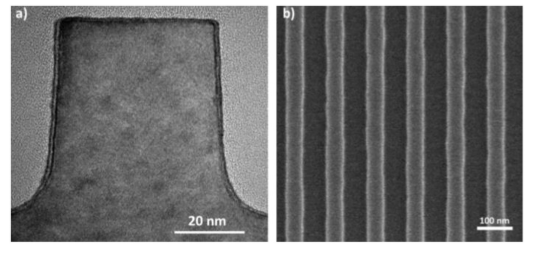
\includegraphics[width=0.6\textwidth]{images/example_structures.png}
    \caption{Examples of nanostructures that is typically being studied for characterisation. a is cross section of a line in b. \cite{rugosity}}
    \label{fig:typical_analyse}
\end{figure}

\medskip

CD-SAXS, a promising technique for nanostructure electronics, uses a transmission geometry, sending the beam through the sample and the 750 micrometer-thick silicon wafer. The x-ray spot size varying between 10-1000 $\mu$m, it enable the measurement of small patterned areas. 
Studies have shown CD-SAXS effectiveness in characterizing the shape and spacing of nanometer-sized patterns \cite{sunday_2015}.

\medskip
CD-SAXS utilizes variable-angle transmission scattering. By rotating the sample, it can probe the vertical profile of the nanostructures. This allows 
for reconstructing their shape and composition in two or even three dimensions.
We can think of it as a diffraction experiment for single crystals, but instead of a crystal, the 
periodic array of nanostructures acts like one. This technique excels at reconstructing 
intricate shapes smaller than 15 nm and with spacing around 30 nm, dimensions crucial for 
the semiconductor industry. \cite{first_cdsaxs_article}

\medskip
While CD-SAXS was demonstrated very useful, the main limitation is inherent to its geometry. The beam needs to go through the 750 micrometer-thick silicon wafer.
This is critical for x-ray energy below 17 keV because a major part of the beam is absorbed. The first CD-SAXS studies were conducted in synchrotron where the energy
of the x-rays can be tuned and where the brilliance is the highest. For laboratory sources, it is currently still an issue since there is no source with enough photons to enable
efficient laboratory measurements. This is a major constrain for the spread of CD-SAXS where a tool in the factory is required to have a direct control during the production. 

\medskip
A possibility to go around the absorption limitation is to perform grazing-incidence experiment where the beam is now reflected at the surface of the sample. This technique, 
called GISAXS become more relevant. It uses X-rays near the critical angle of the probed film resulting in a large sampling area and statistically significant data. This large area allows for faster measurements, enabling in situ kinetic studies.
It has the same resolution of CD-SAXS but enable to examine nanostructures across large areas, i.e. the beam footprint on the sample surface 
being the beam size divided by the sinus of the incident angle of the beam on the sample. For GISAXS, the incident angle is usually around 0.3 deg, making a 10 $\mu$m beam footprint equal to 2 mm for semiconductors. 

\medskip
Early research on X-ray characterization of patterned nanostructures used reflection
methods like X-ray diffraction (XRD) and grazing-incidence small-angle X-ray scattering (GISAXS). 
These techniques demonstrated X-rays sensitivity to features shape and spacing.
Furthermore, X-rays can probe buried features due to their sensitivity to electron density contrast. For instance, a GaInAs/InP multilayer was studied with high-resolution XRD, revealing 
the sensitivity to both the grating and strain between layers \cite{Baumbach_Lübbert_Gailhanou_2000}.

\medskip

While probing large areas is interesting for some application such as the study of polymer for example, it is a limit for 
the semiconductor metrology. Indeed, the patterned areas are only few micrometers wide except for some specific applications like memory arrays (Hofmann et al.,
2009; Scholze et al., 2011). Logic devices require smaller probing areas due to test structure 
size and the complexity of the multicomponent, 3D nanostructures. But CD-SAXS has no such limitation thus it has remerged as a technique that still needs to be developed but is a promising one.\cite{phd_freychet}

\medskip




\subsection{Experimental Setup}

During this project, I had the opportunity to work and observe how CD-SAXS 
measurements are performed at the European Synchrotron Radiation Facility (ESRF)
in Grenoble, France. The ESRF is a world-renowned research facility that provides
intense X-ray beams for a wide range of scientific experiments. Specifically,
I worked with the BM02 beamline, which is dedicated to X-ray scattering and diffraction experiments.

\begin{figure}[h]
\centering
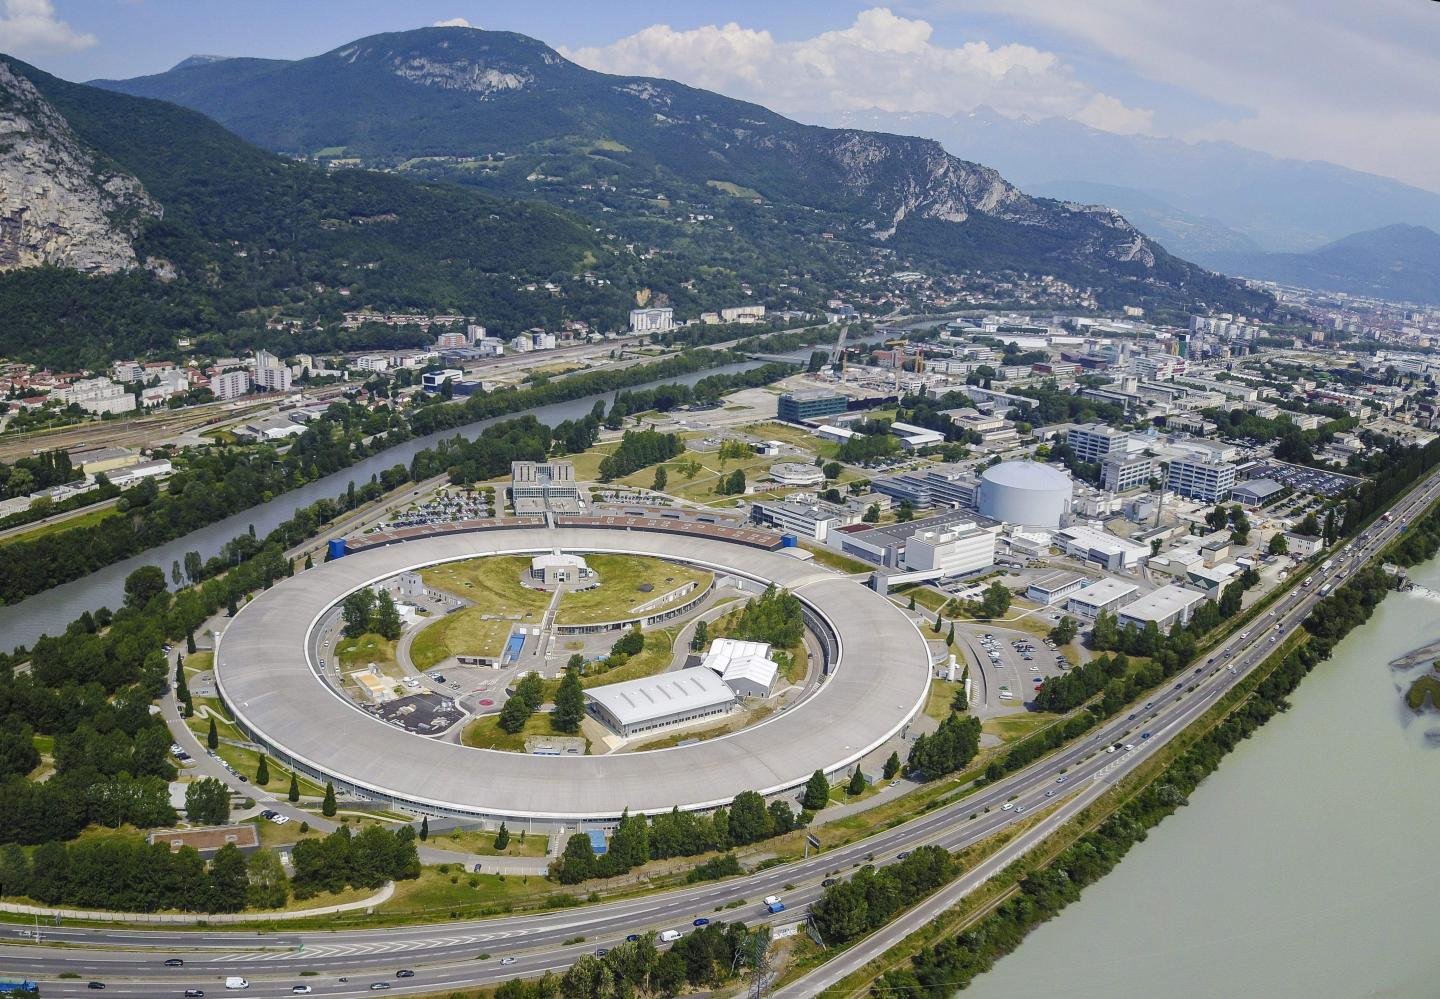
\includegraphics[width=0.6\textwidth]{images/esrf.jpg}
\caption{The European Synchrotron Radiation Facility (ESRF) in Grenoble, France. (credit: ESRF/Jocelyn Chavy)}
\label{fig
}
\end{figure}

The X-ray source obtained from the synchrotron is monochromatized and then focused using
various optical elements. The beam is then directed towards the sample. The 
sample is mounted on a device that allows for rotation and translation in all 
three dimensions. Once the alignment is complete, the sample is rotated along the vertical axis (along the direction of the line), from -60
to 60 degrees with 1 degree step. The scattered X-rays are collected through a detector in a 
vacuum chamber. The data then is interpolated and curve for Intensity vs $Q_{z}$ is extracted for fitting. The schematic of the experiment is shown in Figure \ref{fig:exp_setup},
and the actual experimental setup is depicted in Figure \ref{fig:exp_setup_real}.

\medskip

One of the major challenges in the experiment is the alignment of the sample. Since the area of interest is small, roughly a mm by a mm,
the sample needs to be perfectly positioned at the center of the rotation. Then the rotation axis is brought to the beam position. 
The goal is to keep the same area sample in the sample while rotating. This is achieved by 
aiming a camera at the sample and focusing on the beam position. A short measurement is then performed to observe the diffraction pattern of the sample.
The sample is adjusted until the diffraction pattern is horizontal and centered.

\begin{figure}[h]
\centering
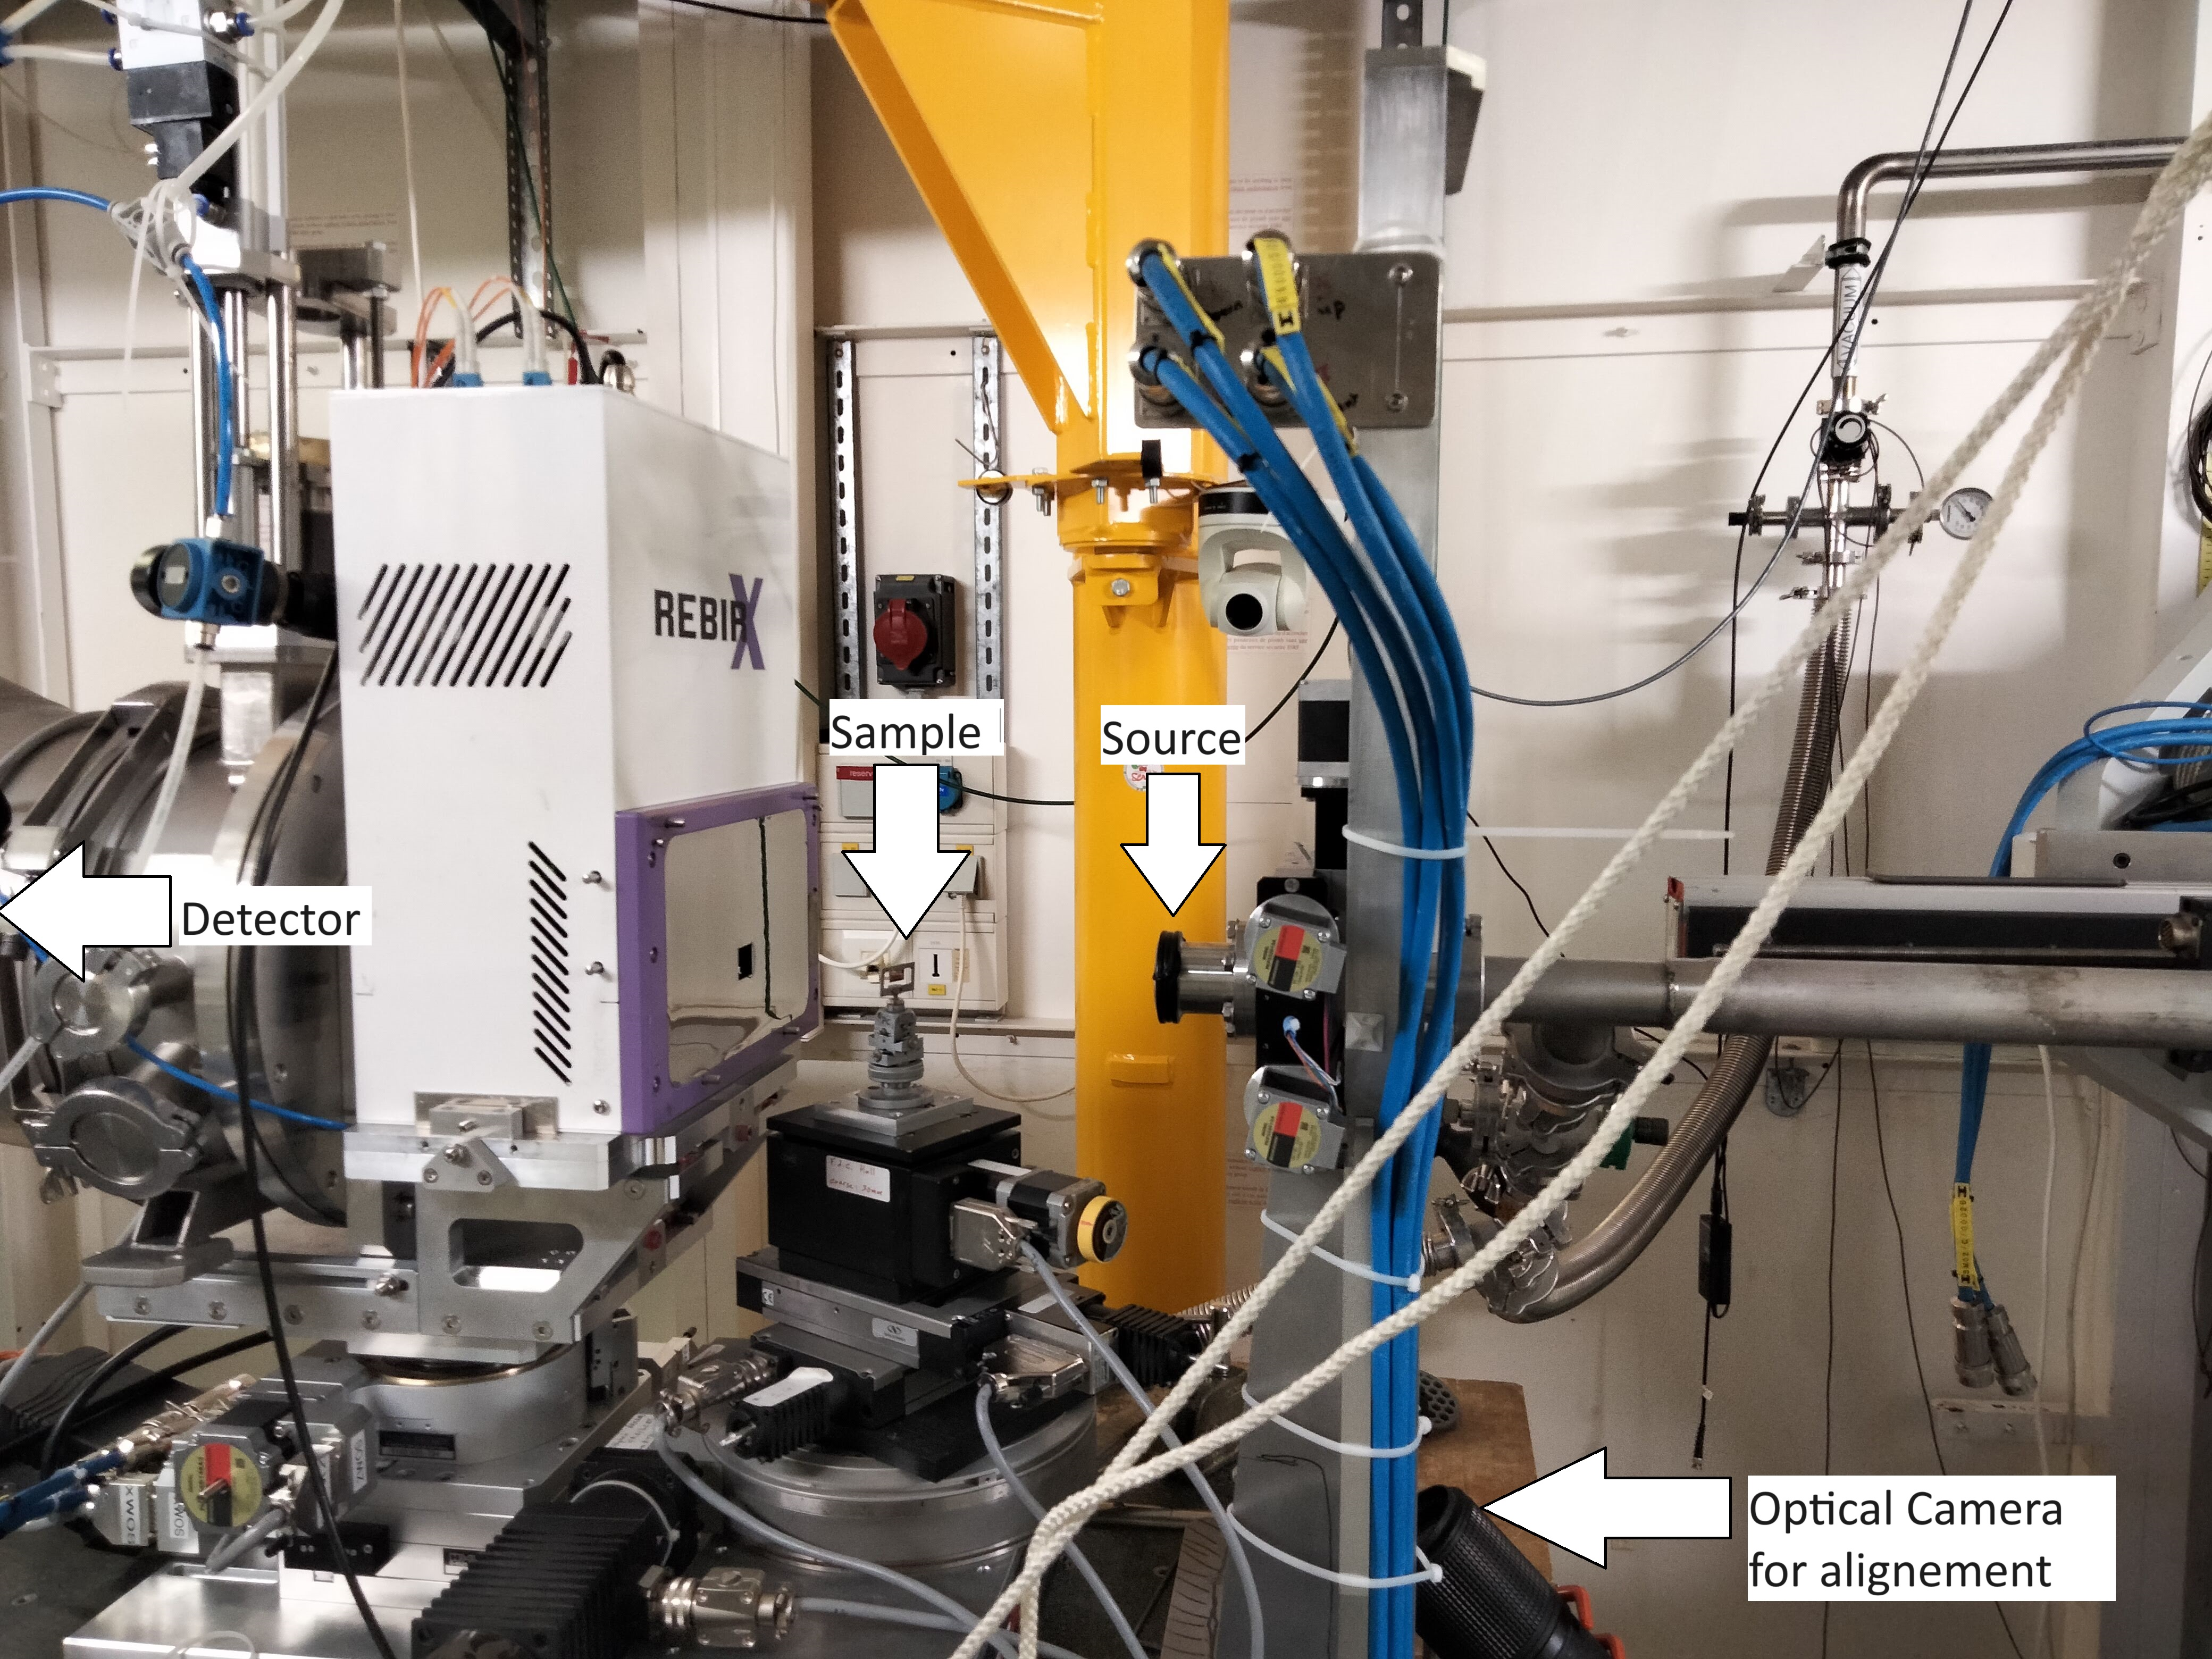
\includegraphics[width=0.6\textwidth]{images/photo_exp.jpg}
\caption{Picture of the experimental setup at the BM02 beamline at ESRF.}
\label{fig:exp_setup_real}
\end{figure}% talk about the alignement problem and how it was solved

\begin{figure}[h]
    \centering
    \begin{minipage}{0.6\textwidth}
        \centering
        \begin{subfigure}[b]{\textwidth}
            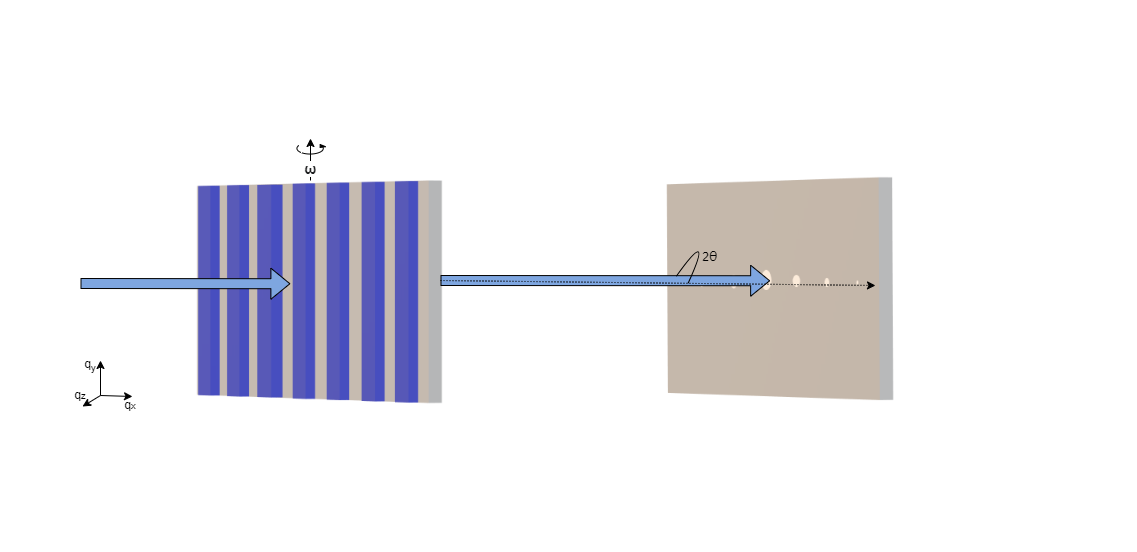
\includegraphics[width=\textwidth]{images/cdsaxs_diff.png}
            \caption{Experimental setup}
            \label{fig:exp_setup}
        \end{subfigure}
    \end{minipage}%
    \hfill
    \begin{minipage}{0.4\textwidth}
        \centering
        \begin{subfigure}[b]{\textwidth}
            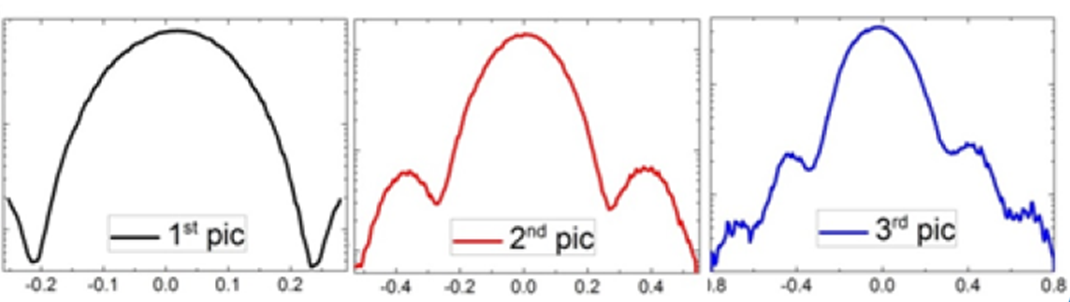
\includegraphics[width=\textwidth]{images/intensity_qz.png}
            \caption{The sample is rotated to get various cuts in the reciprocal space}
        \end{subfigure}
    \end{minipage}
    
    \begin{minipage}{0.5\textwidth}
        \centering
        \begin{subfigure}[b]{\textwidth}
            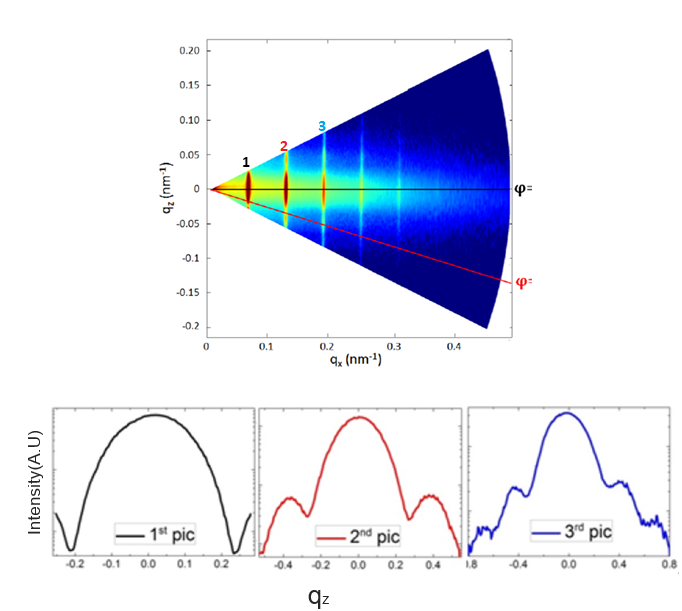
\includegraphics[width=\textwidth]{images/rotation.png}
            \caption{The obtained data is interpolated and data for fitting is extracted}
        \end{subfigure}
    
    \label{fig:exp_setup_concept}
    \end{minipage}
    
    \caption{CD-SAXS instrument layout: X-ray beam passes through the sample, with scattered 
    intensity measured by a 2D detector and converted to $I(Q_{x})$. Measurements at various 
    angles $(\omega)$ are converted, showing intensities as $I$ vs. $Q_{Z}$.}
    \label{fig:isolated_line}
\end{figure}

\FloatBarrier

\subsection{Scattering Model} \label{sec:scattering_model}

\medskip
We will not delve into the complete theory of SAXS here, as it exceeds the scope of this document. 
However, Chapters 1 and 2 of this book \cite{bookSaxs} offer excellent detailed insights into the underlying 
theory. Building upon this, we will now describe the diffraction of a collimated X-ray beam as follows:
\begin{equation}
    I(\mathbf{Q}) = \varOmega | \mathcal{F}(\mathbf{Q}) |^2,
\end{equation}

where $I(\mathbf{Q})$ represents the scattered intensity as a function of the scattering
vector $\mathbf{Q}$, $\Omega$ is a variable independent of $\mathbf{Q}$,
and $\mathcal{F}(\mathbf{Q})$ is the Fourier transform of a function describing the electronic density
distribution within the nanoimprinted pattern.

This relationship is considered valid within the limitations of the CD-SAXS geometry,
which includes a transmission geometry and a low probability of multiple scattering.
Unfortunately, the measured intensity is the absolute square of the Fourier transform. Therefore 
there is a loss of the phase information, making it impossible to analytically extract $F(\mathbf{Q})$ from $I(\mathbf{Q})$.
Therefore, the primary method for determining feature dimensions involves constructing
a real-space model of the pattern cross-section. The Fourier transform of this 
model is then fitted to the experimental CD-SAXS data.

\medskip

During my work-study program, we were mainly concerned with a periodic array of lines, referred to line gratings afterwards (see figure \ref{fig:isolated_line}). The cross-section of
these lines can be represented as a stack of trapezoids (see figure \ref{fig:trapezoid_model}).

\begin{figure}[h]
    \centering
    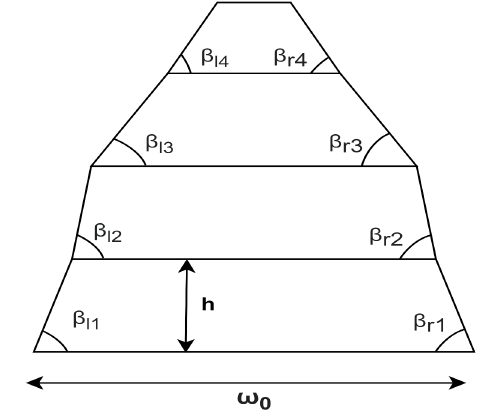
\includegraphics[width=0.3\textwidth]{images/trapezoid.png}
    \caption{Cross-section of a nanostructure line represented as a stack of trapezoids.}
    \label{fig:trapezoid_model}
\end{figure}

The analytical Fourier transform of a trapezoidal shape can be calculated with the following expression \cite{sunday_2015}:
\begin{equation}
    F\left(q_{x}, q_{z}\right)=\frac{1}{q_{x}}\left[-\frac{m_{1}}{t_{1}} e^{-i q_{x}\left(\frac{\omega_{0}}{2}\right)}\left(1-e^{-i h\left(\frac{q_{x}}{m_{1}}+q_{z}\right)}\right)\right. \\ +\frac{m_{2}}{t_{2}} e^{-i q_{x}\left(\frac{\omega_{0}}{2}\right)}\left(1-e^{\left.-i h\left(\frac{q_{x}}{m_{2}}+q_{z}\right)\right)}\right]
    \label{eq:trapezoidal_ft}
\end{equation}
where,

\( \begin{array}{l}\mathrm{m}_{1}=\tan \left(\beta_{1}\right) \\ m_{2}=\tan \left(\pi-\beta_{r}\right) \\ t_{1}= q_{x}+m_{1} q_{z} \\ t_{2}= q_{x}+m_{2} q_{z}\end{array} \)

The different parameters used in the equations are illustrated in figure \ref{fig:trapezoid_model}.
The $\beta$s represent the side wall angle of the trapezoid, $\omega_{0}$ is the line width and $h$ is the 
height of the trapezoids. 

\medskip

so,
\begin{equation}
    I_{0}(\mathbf{q}) = |F(q)|^{2}
\end{equation}

Our analytical model predicts a perfect shape. In order to take into account defects inherent to the lithography process, 
additional factors are introduced to account for an additional decay of scattered intensity $I(Q_{x})$.
These defects can be illustrated as variations a distribution in the in-depth line profile. 
Two main distributions are considered:
\begin{itemize}
    \item \textbf{Random variations in average line position}: the in-depth line profile remains identical along the entire line
         but the average position of the line fluctuates slightly across the whole sample.
    \item \textbf{Variations in the in-depth line profile}: the in-depth line profile itself varies.
\end{itemize}

Both factors indicate a degree of long-range order within the pattern. Additionally, they provide insights into specific types of line edge roughness \cite{these_reche}.
To account for this distribution, we introduce an effective Debye-Waller factor, similar to the one used for fluctuations in crystal lattices.

Hence,

\begin{equation}
    I(\mathbf{q}) = I_{0}(\mathbf{q}) \exp(-q^{2}DW^{2} )
\end{equation}

where $DW$ is the Debye-Waller factor.

\subsection{Fitting Algorithm}

While CD-SAXS excels at detecting deviations from a perfect grating pattern in buried structures, it requires 
additional processing to convert the raw data into a meaningful real-world structure. This process involves using 
an inverse algorithm, which essentially translates the scattered intensity information back into the original structures 
characteristics.

\medskip

CD-SAXS measurements provides experimental data. The objective of the inverse fitting is to iterate over a high number of different line profile (represented as various combination of stacked trapezoids)
and to converge towards the profile that its Fourier Transform will best match the experimental data. While the objective seems simple to describe, 
the problem is complex. Traditional optimization methods used for refinement often fall short when dealing with 
complex internal structures with numerous parameters, either being trapped in local minima or not converging toward the same solutions.

\medskip

Another challenge arises from the possibility of "degenerate" solutions. These occur when multiple structural 
models can produce the same scattering data, making it difficult to pinpoint the true structure. This is a common 
issue in scattering analysis.

\medskip

Therefore, the ideal scenario for CD-SAXS analysis involves an optimization algorithm that can consistently and 
rapidly converge on the best possible fit for the data. While some prior knowledge about the underlying structure 
can accelerate the process, such information is not always readily available. This highlights the need for more 
efficient algorithms that can handle complex structures even with limited prior knowledge.

\medskip

Previous research has explored various algorithms to determine the optimal set of parameters for a model that 
best fits the experimental CD-SAXS data. These parameters essentially describe the nanostructure 
being analyzed.

\medskip

One approach utilizes a Markov chain Monte Carlo (MCMC) algorithm. However, this method requires a good initial 
guess for the structure parameters and limitations on their search range. Additionally, it necessitates multiple 
independent runs to ensure that the algorithm converges on the correct solution. While this approach can be effective, 
the need for tight parameter bounds might overlook potential fabrication errors in the sample.

\medskip

Another strategy involves massive computing resources with parallelization and highly refined grid-based models. 
This method, known as reverse MCMC, offers greater accuracy but is limited by the availability of such computational power.

\medskip

Genetic and evolutionary algorithms have emerged as promising alternatives. These methods mimic biological evolution, 
with the model parameters acting as the "genetic code." Starting with randomly generated parameters, these algorithms 
iteratively refine them through a "mixing strategy" over multiple generations until the optimal set is found. This 
approach excels at searching large parameter spaces with wide bounds, making it suitable for complex structures.
\cite{hannon2016advancing}

\subsubsection{Covariance Matrix Adaptation Evolution Strategy (CMAES)}

One algorithm is the Covariance Matrix Adaptation Evolution Strategy (CMAES). This method is particularly 
well-suited for high-dimensional optimization problems, making it ideal for complex nanostructure analysis. CMAES 
operates by maintaining a population of candidate solutions, with each iteration generating new candidates based on 
the previous generation performance. By adapting the covariance matrix of the candidate solutions, CMAES can efficiently 
explore the parameter space and converge on the optimal solution.

\begin{figure}[h]
    \centering
    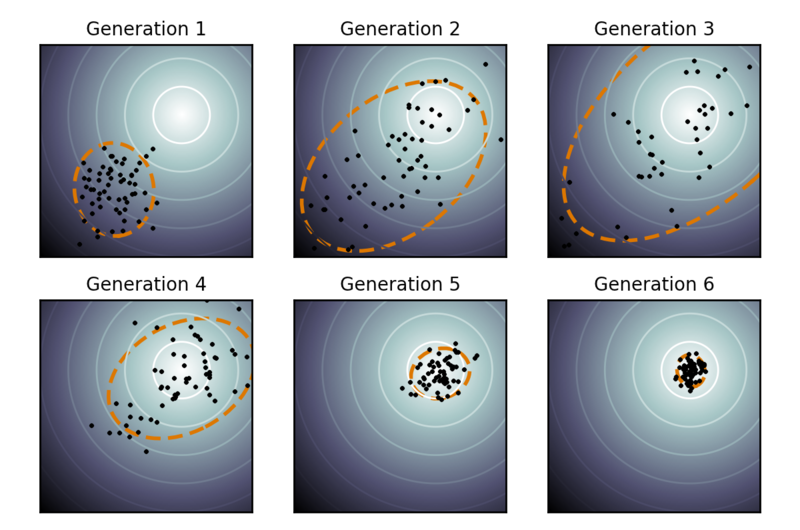
\includegraphics[width=0.8\textwidth]{images/CMAES.png}
    \caption{Illustraion of CMAES algorithm. The algorithm maintains a population of candidate solutions, with each 
    iteration generating new candidates based on the previous generation performance.(image taken from wikipedia CMAES page) }
    \label{fig:cmaes}
\end{figure}

\FloatBarrier

\medskip

For CD-SAXS experiment, the algorithm starts with the experimental data collected. Then, a series of in-depth line profile generated, through a set of parameters as describe earlier. 
Afterwards, the calculated analytical Fourier transform is compared with the experimental data using a mean-absolute error log:

\medskip

\begin{equation}
    \Xi=\frac{1}{N_{\mathrm{q}}-1} \sum_{\mathbf{q}}\left|\log _{10} I_{\mathrm{Sim}}(\mathbf{q})-\log _{10} I(\mathbf{q})\right|
\end{equation}

\medskip

where $I_{\mathrm{Sim}}(\mathbf{q})$ is the simulated intensity and $I(\mathbf{q})$ is the experimental intensity.
$\Xi$ is called goodness of fit. The algorithm then tries to minimize $\Xi$ by adjusting the parameters of the model.

\medskip

In an article \cite{hannon2016advancing}, researchers investigated the efficiency of various algorithms
for reconstructing various nanostructures using X-ray scattering data.
Their findings specifically highlighted the advantages of the CMAES. Compared to other
methods like Markov Chain Monte Carlo (MCMC) and Differential Evolution 
(DE), CMAES demonstrated significantly faster convergence times when 
analyzing an experimental structure. Notably, CMAES reached a solution 
that matched the quality of previous studies in approximately 1 to 2 
orders of magnitude less time than MCMC and less than an order of 
magnitude time than DE. This speed advantage held true regardless 
of the specific objective function used to evaluate the goodness of fit. 
These results suggest that CMAES offers a powerful tool for analyzing 
complex nanostructures with X-ray scattering data, particularly when 
dealing with limited computational resources or tight time constraints.

\subsubsection{Uncertainty estimation by Monte Carlo Markov Chain(MCMC) method}\label{sec:mcmc_cdsaxs}

The CMAES algorithm provides a single best-fit solution for the nanostructure parameters. However, it is essential to understand the uncertainty associated with these parameters.
This uncertainty relates to the different possible combinations of parameters that could result in a similar goodness of fit. 
For instance, decreasing slightly height of one trapezoid and increasing the height of an other one can result in a similar goodness of fit.
To address this, we can use MCMC algorithm to explore and find all the sets of population that can result in the same goodness of fit.

\medskip

This confidence interval then can be calculated from this population of parameters. This interval gives us an idea of the range of possible values for each parameter that could still provide a good fit to the data.
The lower and upper bounds of this interval can be used to estimate the uncertainty associated with each parameter.

\begin{figure}[h]
    \centering
    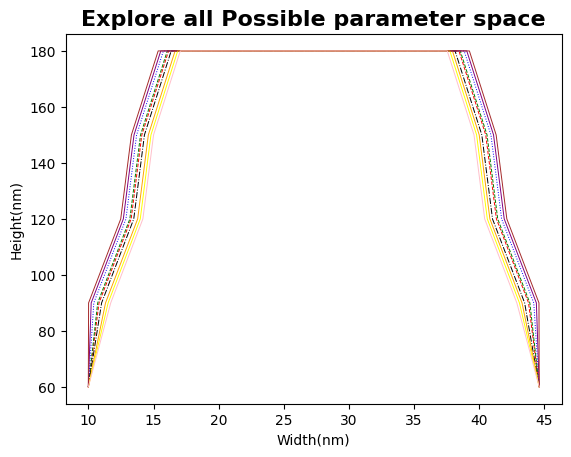
\includegraphics[width=0.5\textwidth]{images/mcmc.png}
    \caption{MCMC algorithm exploring all possible sets of parameters that can result in the same goodness of fit. The different
    colours represent the different set of paramaters that can result in the same goodness of fit.}
\end{figure}
\medskip



After determining the best-fit model structure, the researchers of this article \cite{sunday2016evaluation}
employed a MCMC algorithm to calculate the uncertainties associated with the model parameters.
This algorithm generates a population of models that can be evaluated to assess the uncertainty
in a set of parameters. The probability of a given model being accepted into the population
depends on how well the simulated scattering profile it generates matches the experimentally
measured one.

Here is the overview of the algorithm:

\begin{enumerate}
    \item \textbf{Seeding:} The algorithm initializes with the model (M) exhibiting the best known goodness-of-fit, denoted GFB.
    \item \textbf{Proposal generation:} Random perturbations are applied to each parameter within the model, resulting in a new candidate model (M$_i$) and its corresponding goodness-of-fit GF (GF$_i$).
    \item \textbf{Acceptance for better fit:} If GF$_i$ $<$ GF$_{i-1}$, then M$_i$ is automatically accepted into the population (and GFB is updated to GFB = GF$_i$ if the new model has a better fit).
    \item \textbf{Metropolis-Hastings acceptance for worse fit:} If GF$_i$ $>$ GF$_{i-1}$, the probability (P$_i$) of accepting M$_i$ is calculated using Eq. \eqref{eq:mcmc_acceptance}:
    \begin{equation}
        P_i = \exp \left( -0.5 \cdot (\text{GF}_i - \text{GFB}) \right) \label{eq:mcmc_acceptance}
    \end{equation}
    A random number $\alpha$ between 0 and 1 is then generated. If $\alpha < P_i$, M$_i$ is accepted; otherwise, it is rejected, and a new proposal is generated from M$_{i-1}$.
    \item \textbf{Equilibrium and resampling:} Steps 2-4 are repeated until the model population reaches an equilibrium. To avoid correlations between accepted models, the population is resampled (e.g., every 50 steps in this case).
    \item \textbf{Uncertainty calculation:} The uncertainties are calculated from the final accepted model population and represent a 95\% confidence intervals. The step size for generating proposals was optimized to achieve an
    acceptance probability between 0.25 and 0.35, a range known to yield the fastest convergence.
\end{enumerate}

I used a very similar algorithm but with some modifications to increase the efficiency, we will discuss this in the next section.

\subsubsection{Overall view of the CD-SAXS inverse problem resolution}

\medskip

The process begins with an initial guess for the parameters of the model, which describe a geometric structure with specific width and height parameters. The model data is then transformed into the reciprocal space using a Fourier Transform.
This transformed data is then compared with the experimental data. Finally, the error between the simulated and experimental data is minimize by exploring the parameters space.

\medskip

The error between the experimental and simulated data is quantified using an error metric that measures the goodness-of-fit by comparing the logarithms of the simulated and experimental intensity profiles. If the error is within a tolerable range, the fit is considered acceptable, and the best-fit model is extracted. This involves identifying the parameters that provide the best match to the experimental data.

\medskip

To quantify the uncertainties associated with the fitted parameters, a Monte Carlo approach is employed. This involves exploring the possible parameter space through a series of stochastic simulations. The MCMC method is used to sample the parameter space, ensuring that the distribution of the sampled parameters reflects their likelihood given the data. During the MCMC process, initial samples are generated from the best-fit parameters, new samples are proposed by perturbing the current parameters, and the Metropolis-Hastings criterion is used to decide whether to accept or reject the new samples based on their goodness-of-fit compared to the previous samples. This process is repeated until a sufficient number of samples are collected, ensuring the sampled parameter distribution converges to the true posterior distribution.

\medskip

The final step involves calculating the error bars (uncertainties) for the fitted parameters based on the Monte Carlo samples, providing 95\% confidence intervals and a robust measure of the reliability of the fitted model parameters. By combining CMAES for initial parameter optimization and MCMC for uncertainty quantification, the algorithm offers a robust approach to model fitting, ensuring both optimal parameter estimation and reliable uncertainty analysis.

\medskip

Here is a figure that shows the overall view of the CD-SAXS algorithm:

\begin{figure}[h]
    \centering
    \begin{subfigure}[b]{1\textwidth}
        \centering
        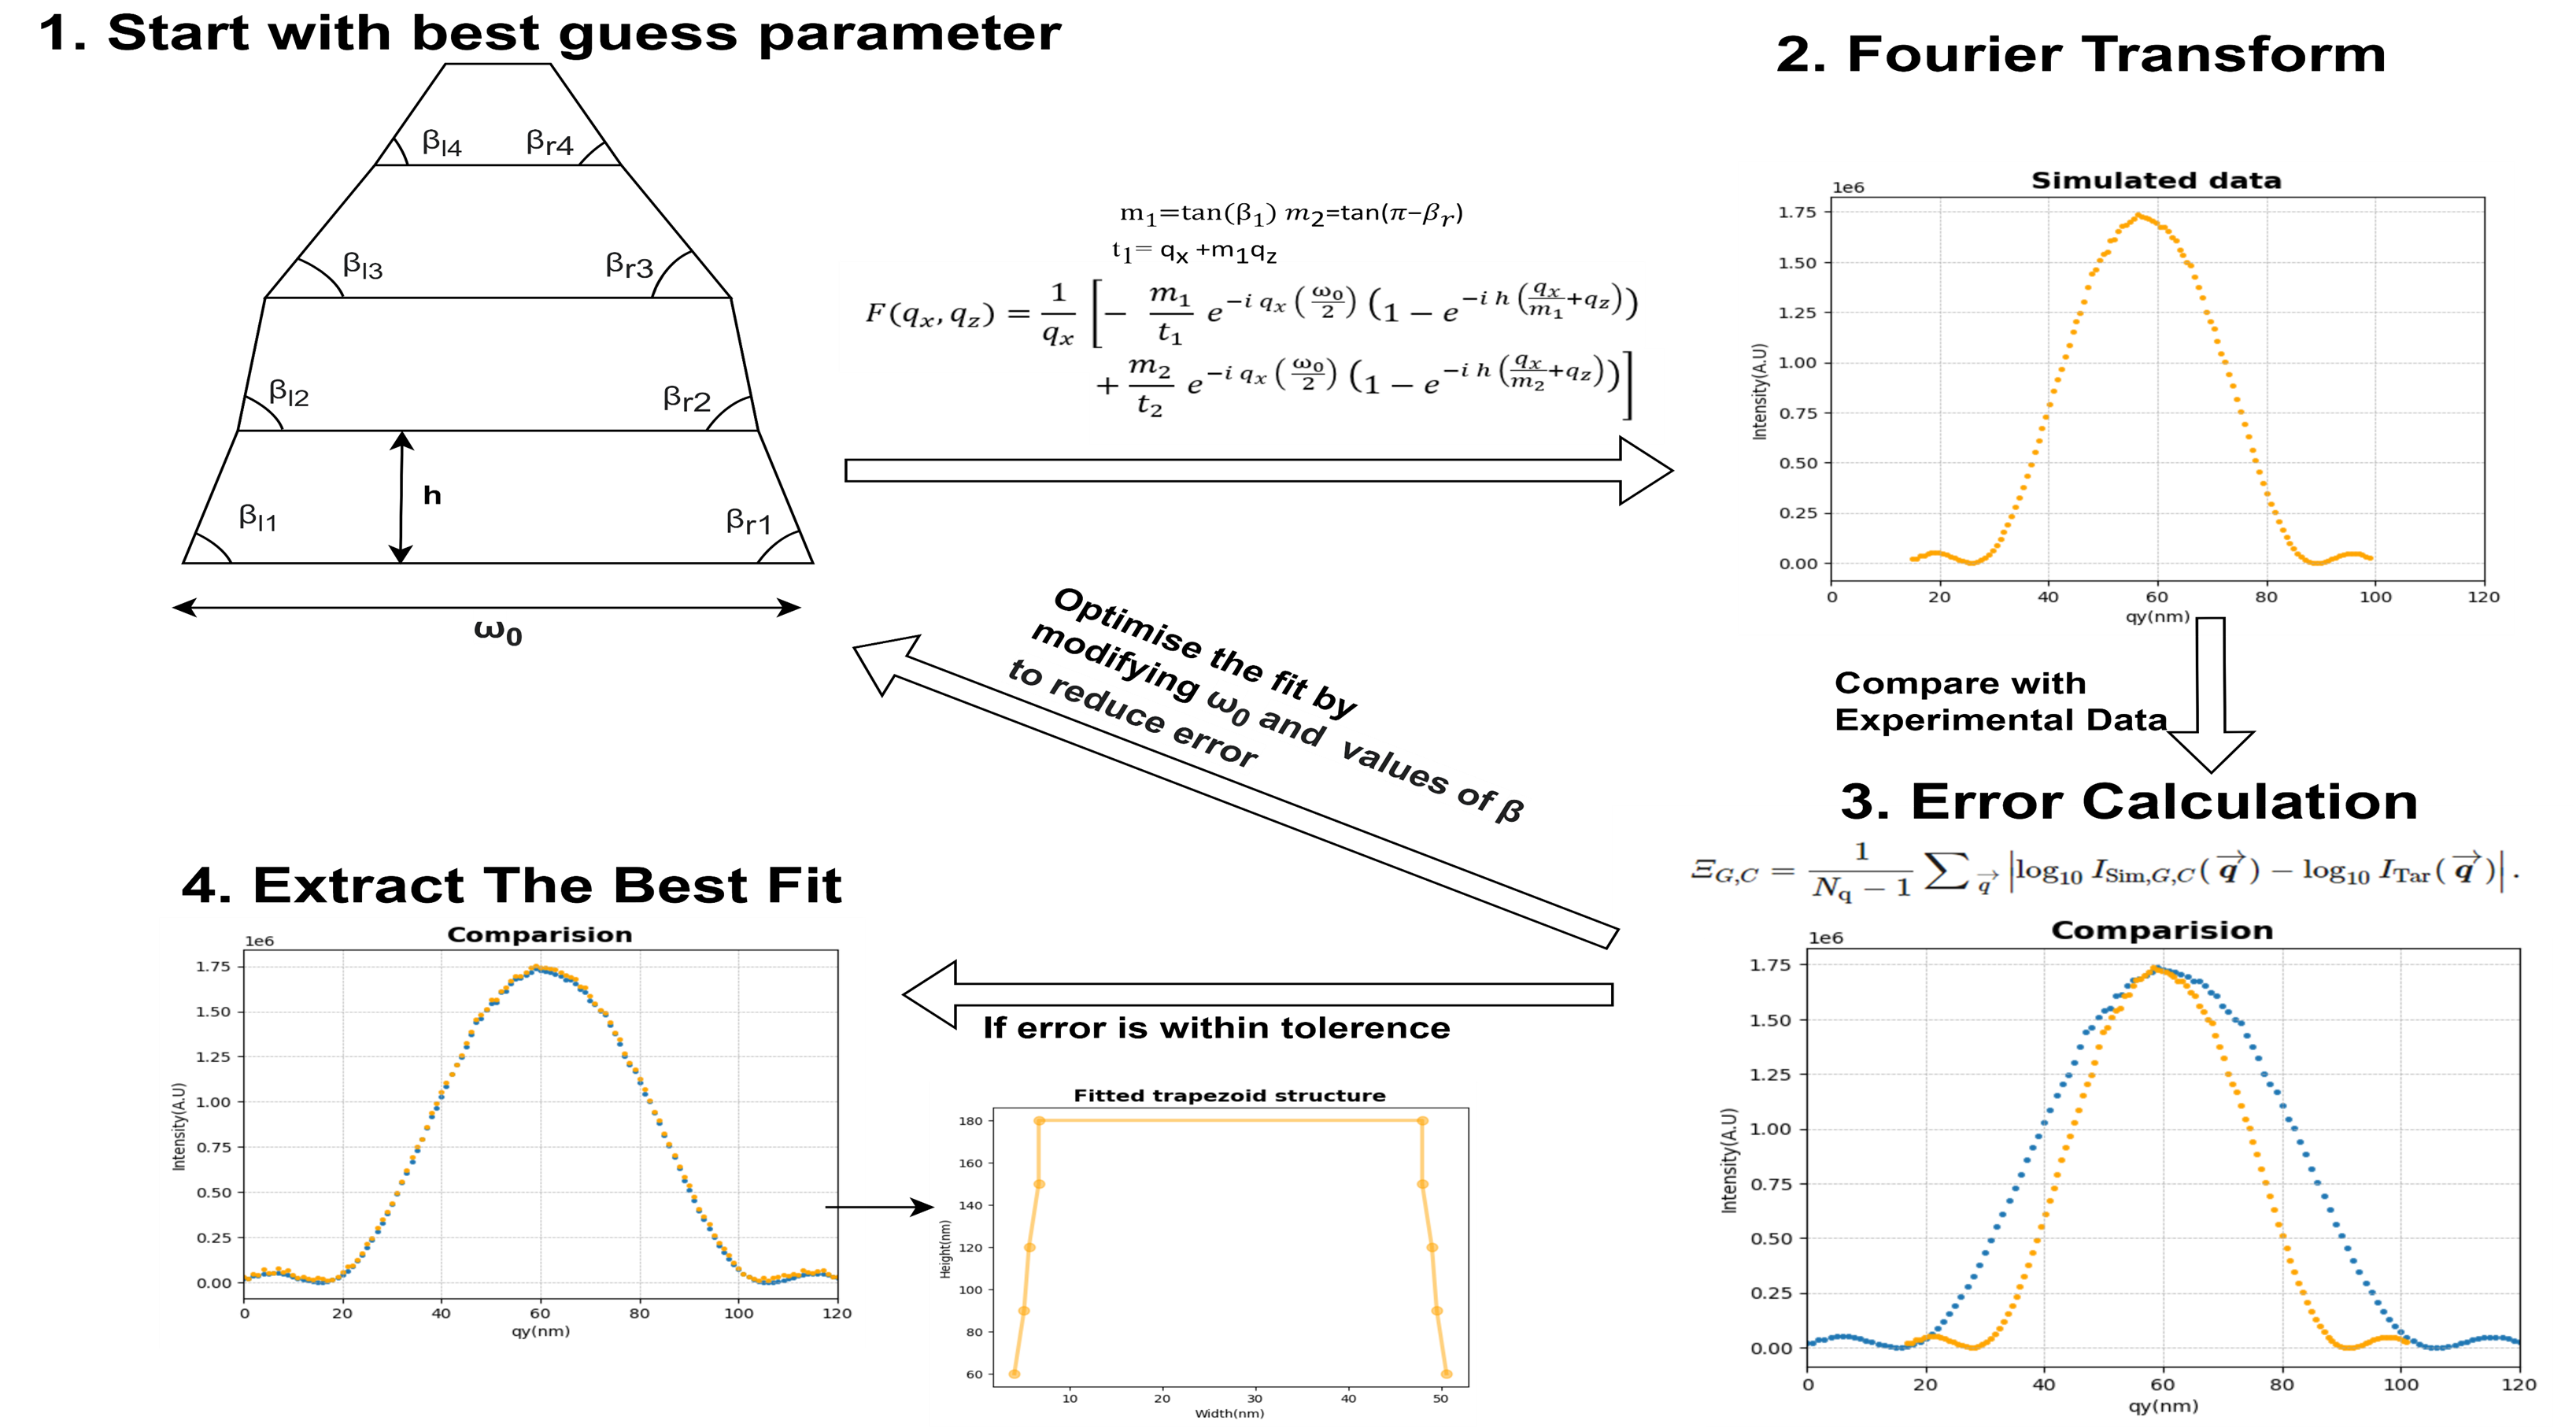
\includegraphics[width=\textwidth]{images/cmaes_overall.png}
    \end{subfigure}
    \\
    \begin{subfigure}[b]{1\textwidth}
        \centering
        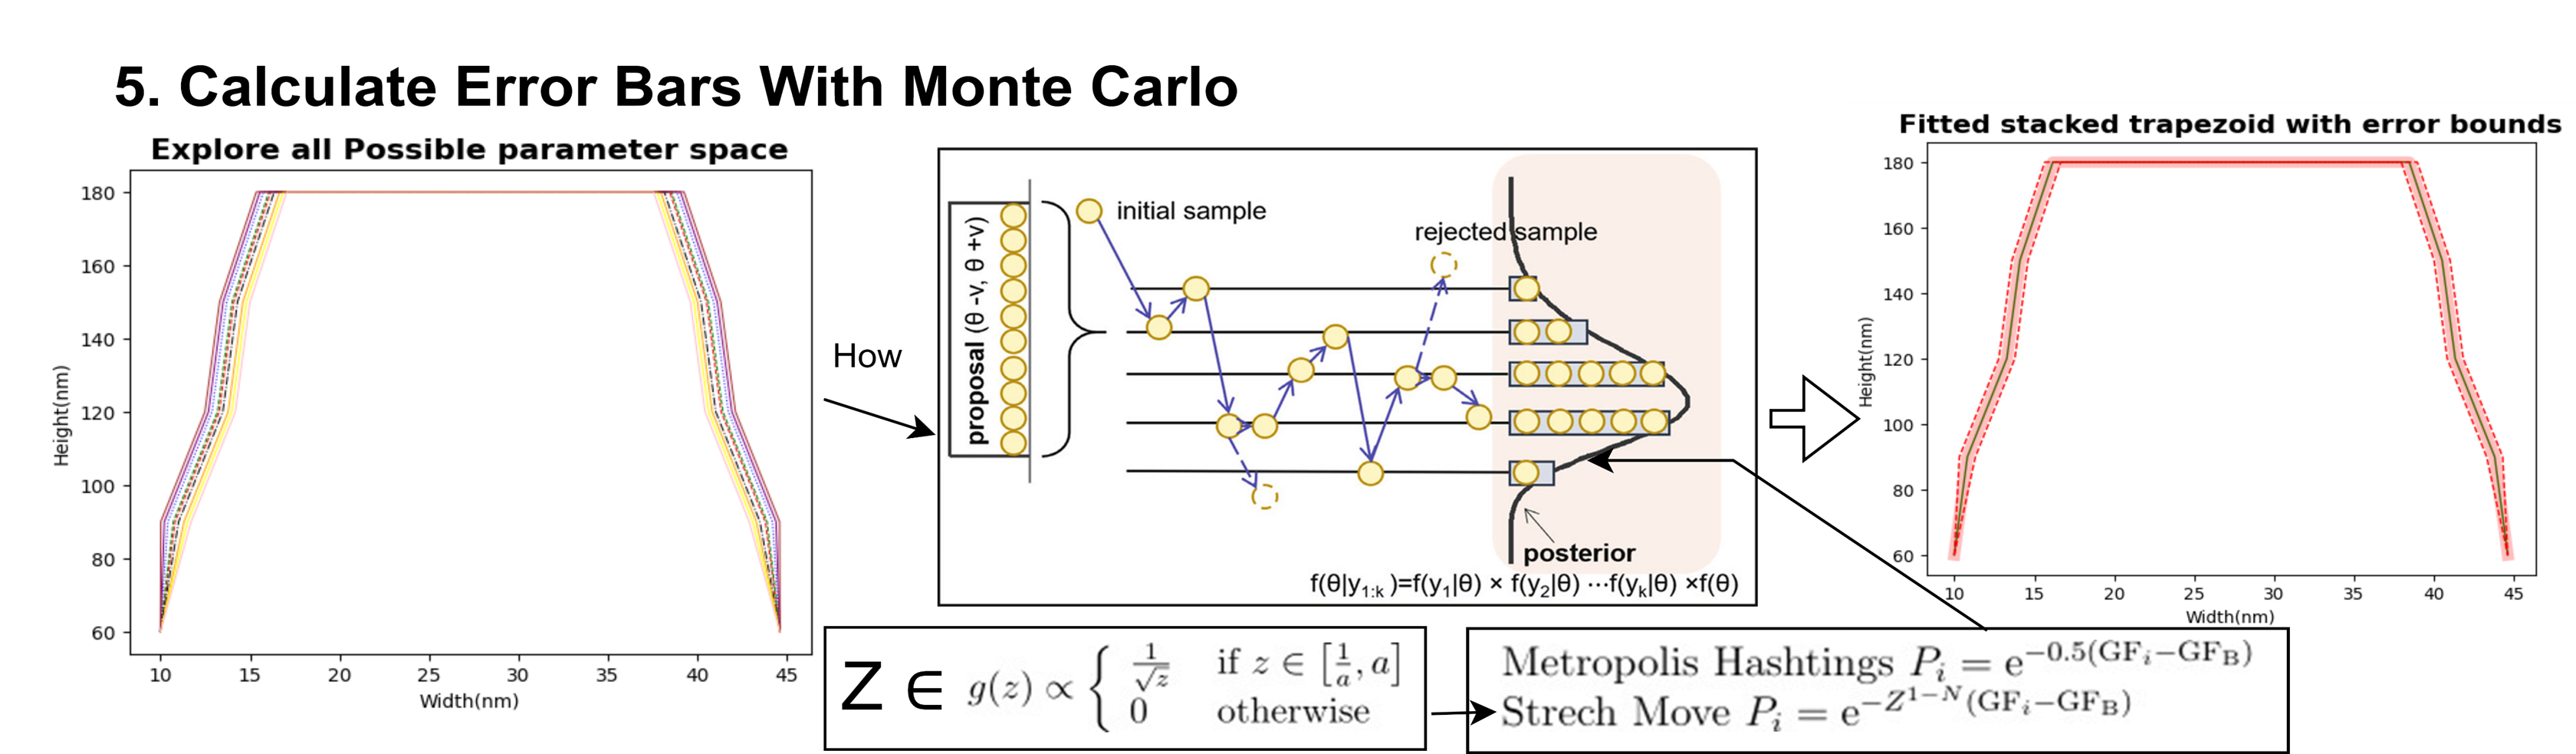
\includegraphics[width=\textwidth]{images/mcmc_overall.png}
    \end{subfigure}
    \caption{Illustration of the different steps and algorithm used during the CD-SAXS analysis. First, CMAES for initial parameter optimization and then MCMC for uncertainty quantification are used.}
    \label{fig:cd_saxs_algo}
\end{figure}

\FloatBarrier


